\documentclass[a4paper]{paper}

\usepackage{amsmath}
\usepackage{amsfonts}
\usepackage{amssymb}
\usepackage{tikz}

\usetikzlibrary{shapes,arrows,positioning}

\begin{document}
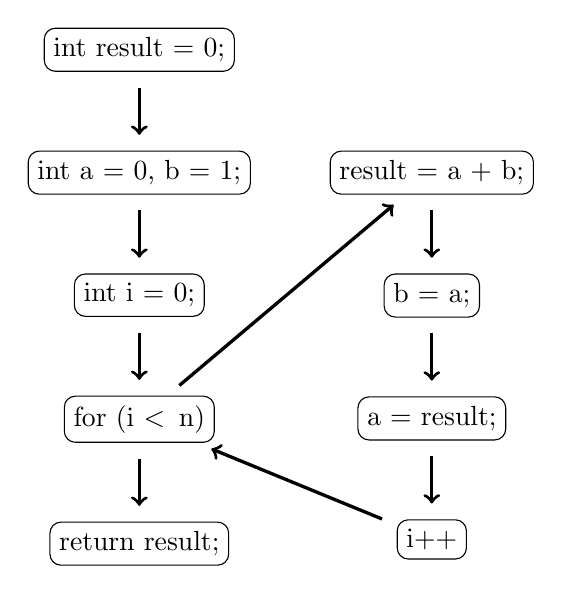
\begin{tikzpicture}%[node/.style = {draw=black, thick, elipse}, node distance=1cm]
    \tikzset{
        n/.style        =   { rectangle
                            , rounded corners
                            , text centered
                            , draw=black
                            }
        , arrow/.style  =   { very thick
                            , shorten >= 0.2cm
                            , shorten <= 0.2cm
                            }
    }
    \node(1)[n] {int result = 0;};
    \node(2)[n,below=of 1] {int a = 0, b = 1;};
    \node(3)[n,below=of 2] {int i = 0;};
    \node(4)[n,below=of 3] {for (i \textless \enskip n)};
    \node(5)[n,right=of 2] {result = a + b;};
    \node(6)[n,below=of 5] {b = a;};
    \node(7)[n,below=of 6] {a = result;};
    \node(8)[n,below=of 7] {i++};
    \node(9)[n,below=of 4] {return result;};

    \draw[arrow,->] (1) -- (2);
    \draw[arrow,->] (2) -- (3);
    \draw[arrow,->] (3) -- (4);
    \draw[arrow,->] (4) -- (5);
    \draw[arrow,->] (4) -- (9);
    \draw[arrow,->] (5) -- (6);
    \draw[arrow,->] (6) -- (7);
    \draw[arrow,->] (7) -- (8);
    \draw[arrow,->] (8) -- (4);
\end{tikzpicture}
\end{document}